% Appendix A

\chapter{Problemas NP y PH modelados en lógica}
\label{apendiceA}
\lhead{Apéndice A. \emph{Problemas NP y PH modelados en lógica}}

*** FALTA UNA DESCRIPCIÓN EN TEXTO DE LA INTUICIÓN DETRÁS DE LA MODELACIÓN DE
CADA DOMINIO, Y EJEMPLOS DE IMÁGENES CON GRAFOS ***

\section{Problemas NP}

\subsection{SAT, Satisfacibilidad proposicional}
Existe una asignación de verdad $T$, tal que para toda cláusula $y$, existe una variable $x$, tal que:
$x$ esta positiva en $y$ y $T(x)$, o $x$ esta negativa en $y$ y $not-T(x)$,
\begin{verbatim}
(so-exists (?T 1)
  (forall (?y)
    (exists (?x)
      (or
        (and (?P ?x ?y)
             (?T ?x)) 
        (and (?N ?x ?y)
             (not (?T ?x)))))))
\end{verbatim}

\subsection{CLIQUE, Clique de tamaño $k$}

\begin{verbatim}
(so-exists (?F Inj)
  (and (forall (?y) (exists (?x) (?F ?x ?y)))  ; totality
    (forall (?x) (forall (?y)
      (implies (and (< ?x ?y)
                    (exists (?z) (and (?F ?x ?z) (?K ?z)))
                    (exists (?z) (and (?F ?y ?z) (?K ?z))))
               (?E ?x ?y))))))
\end{verbatim}
\begin{figure}[h!]
\centering
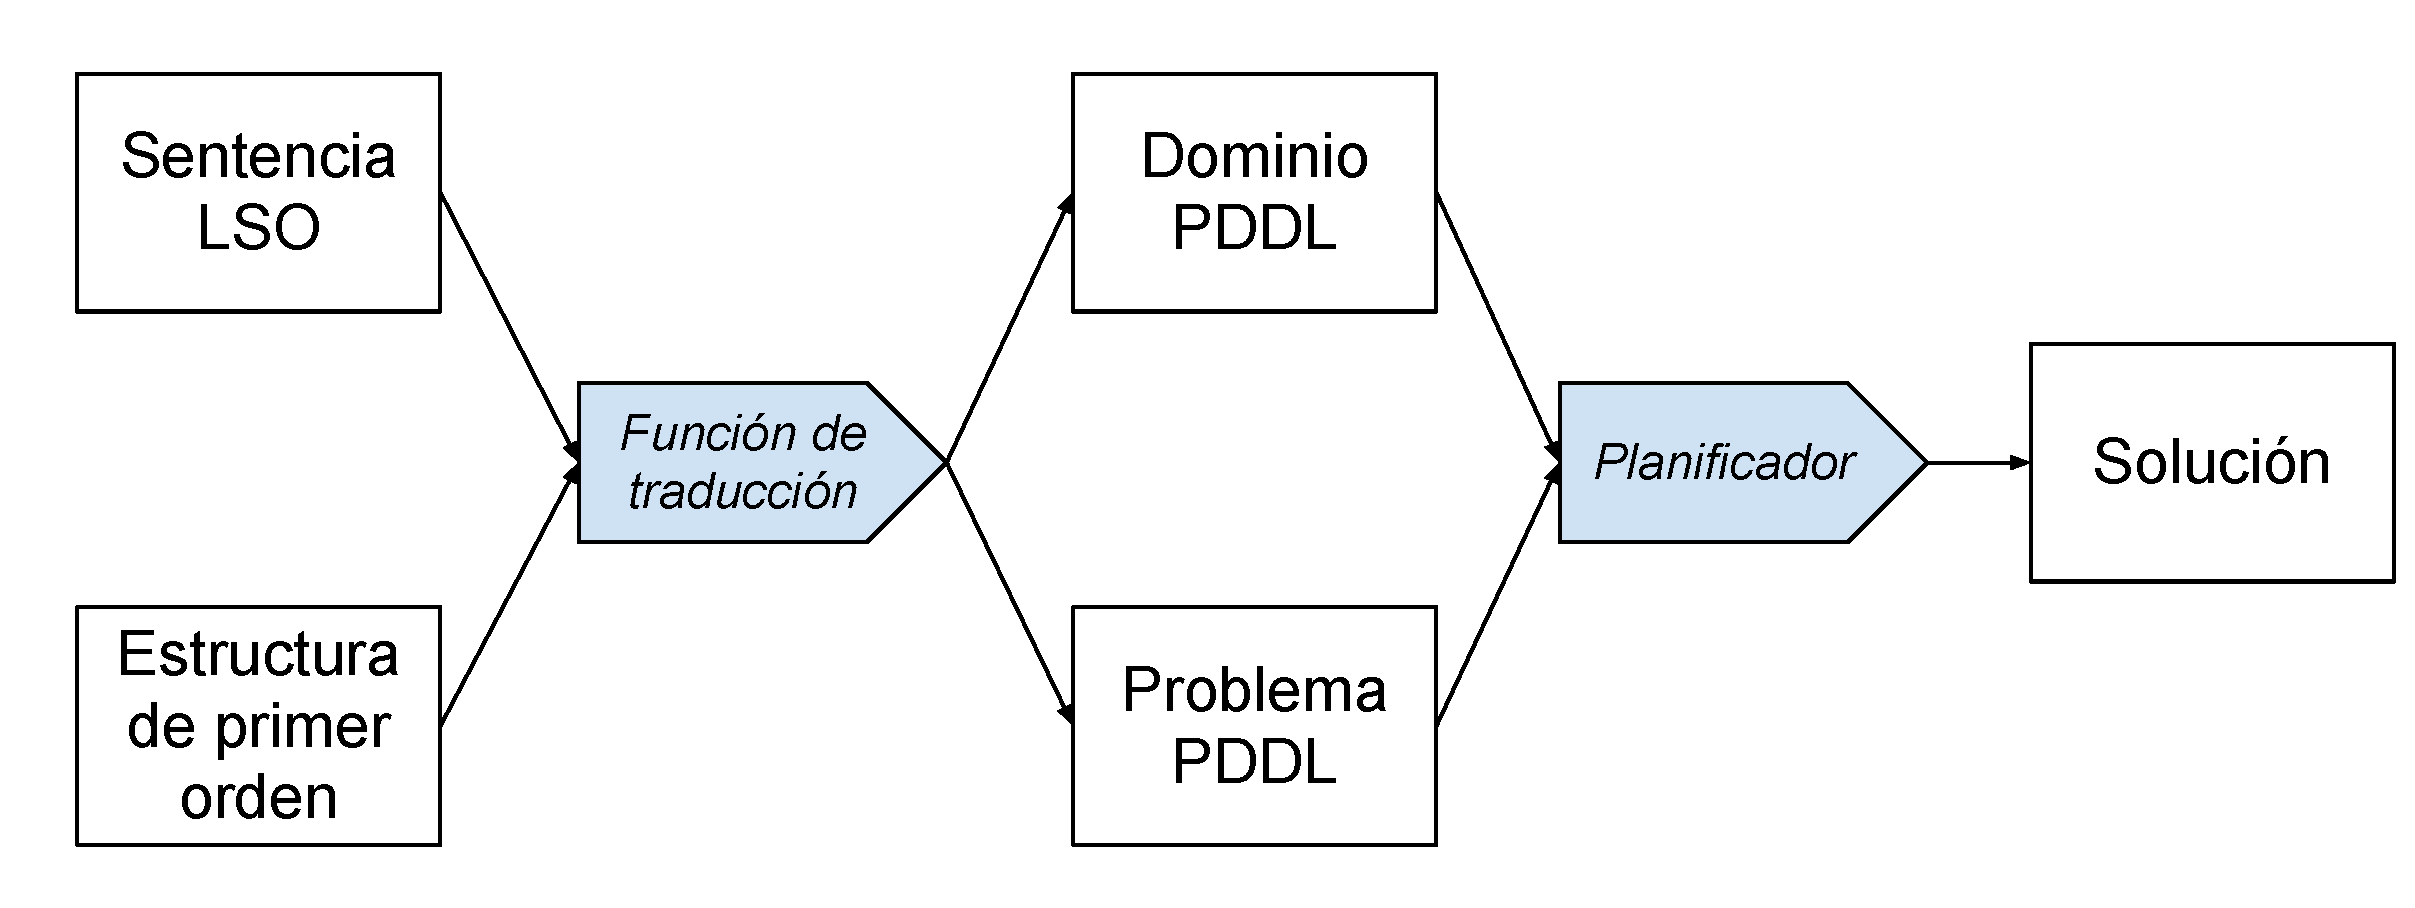
\includegraphics[width=\textwidth]{figuras/esquema_herramienta.pdf}
\caption[Grafo con una \textit{clique} de tamaño $k = 6$]{Grafo con una clique de tamaño
$k = 6$}
\label{clique}
\end{figure}

\begin{verbatim}
(exists F in Inj)(forall x y)[f(x) < K & f(y) < K -> E(x,y)]
\end{verbatim}

\subsection{\CHD, Camino Hamiltoniano Dirigido}
Esta fórmula expresa que existe una manera ordenada $F(a,b)$ de visitar los nodos de grafo (la posición $a$ la tiene el nodo $b$), en
la que para toda posición $x$, si no es la última, entonces existe un nodo $y1$ que le corresponde esta posición, y además
a la siguiente posición $x2$ le corresponde otro nodo $y2$, y hay un arco entre $y1$ y $y2$.
\begin{verbatim}
(so-exists (?F Inj)
  (forall (?x)
    (implies (< ?x MAX)
             (exists (?y1)
               (and (?F ?x ?y1)
                 (exists (?y2)
                   (and
                     (exists (?x2) 
                       (and (SUC ?x ?x2) (?f ?x2 ?y2)))
                   (?E ?y1 ?y2))))))))
\end{verbatim}
\begin{verbatim}
; (exists F in Inj)(forall x)[x < MAX -> E(f(x),f(x+1))]
\end{verbatim}

\subsection{\TDM, \textit{3-Dimensional Matching}}
\begin{verbatim}
(so-exists (?F Inj)
  (so-exists (?G Inj)
    (and
      (forall (?x) (exists (?y) (?F ?x ?y))) ; F is total
      (forall (?x) (exists (?y) (?G ?x ?y))) ; G is total
      (forall (?x) (forall (?y) (forall (?z)
        (implies (and (?F ?x ?y) (?G ?x ?z))
                 (?T ?x ?y ?z))))))))
\end{verbatim}

\subsection{\TCOL, 3-colorabilidad}
Esta fórmula expresa que existe una asignación de colores $R$, $G$ y $B$ tal que para todos los nodos
de un grafo, no hay dos vertices adyacentes del mismo color, los vertices tienen
almenos y a lo sumo un color.
\begin{verbatim}
(so-exists (?R 1) (so-exists (?G 1) (so-exists (?B 1)
  (forall (?x) 
    (and
      ; no hay dos vértices adyacentes del mismo color
      (forall (?y)
        (implies (?E ?x ?y) (not (or (and (?R ?x) (?R ?y))
                                        (and (?G ?x) (?G ?y))
                                        (and (?B ?x) (?B ?y))))))

        ; los vértices tienen al menos un color
        (or (?R ?x) (?G ?x) (?B ?x))

        ; los vértices tienen a lo sumo un color
        (implies (?R ?x) (and (not (?G ?x)) (not (?B ?x))))
        (implies (?G ?x) (and (not (?R ?x)) (not (?B ?x))))
        (implies (?B ?x) (and (not (?R ?x)) (not (?G ?x)))))))))
\end{verbatim}

\subsection{\KCOL, k-colorabilidad}
Esta fórmula expresa que existe una función de asignación de colores $F$, tal que a todo nodo se le es
asignado un color $y$, donde $K(y)$ quiere decir que el color $y$ es menor al máximo color
$k$; ademá, para todos los otros nodos, si este esta conectado a ellos, no
tienen el mismo color.

\begin{verbatim}
(so-exists (?F Func)
  (forall (?x) 
    (and (exists (?y) (and (?F ?x ?y) (?K ?y)))
      (forall (?y) 
        (implies (?E ?x ?y)
                 (not (exists (?z)
                   (and (?F ?x ?z) (?F ?y ?z)))))))))
\end{verbatim}

\section{Problemas PH}

\subsection{UNSAT, No-Satisfacibilidad proposicional}
Esta fórmula expresa que para toda relación $T$ sobre variables
proposicionales, existe una cláusula $y$ tal que para cada variable $x$, o $x$
aparece positiva en $y$ y $x$ es falsa, o $x$ aparece negativa en $y$ y $x$ es
verdadera, o $x$ no aparece en $y$.
\begin{verbatim}
(so-forall (?T 1 @ist)
    (exists (?y @cls)
        (forall (?x @var)
            (or (and (?N ?x ?y)
                     (?T ?x)
                )
                (and (?P ?x ?y)
                    (not (?T ?x))
                )
                (?NotIn ?x ?y)
             ))))
\end{verbatim}

\subsection{\qEA-QBF, Fórmula \textit{booleana} cuantificada $\Sigma_p^2$}
Esta fórmula expresa que existe una relación $E0$ sobre variables
proposicionales, tal que para toda relación $A0$ sobre variables
proposicionales, Para toda cláusula $c$ existe una variable $x$, tal que: o $x$ aparece
positiva en $c$ y es verdadera existencial o universalmente, o $x$ aparece negativa en $c$ y
es negativa existencial o universalmente.
\begin{verbatim}
(so-exists (?E0 1 @ise0)
    (so-forall (?A0 1 @isa0)
        (forall (?c @cls)
            (exists (?x @var)
                (or
                    (and (?P ?x ?c) (?E0 ?x))
                    (and (?P ?x ?c) (?A0 ?x))
                    (and (?N ?x ?c) (not (?E0 ?x)))
                    (and (?N ?x ?c) (not (?A0 ?x)))
                )))))
\end{verbatim}

\subsection{\coCOL, No-3-Colorabilidad}
Esta fórmula expresa que para toda posible coloración de nodos $R$, $G$ y $not-G \land not-R$, o dos nodos unidos por un arco tienen
el mismo color, o un nodo tiene dos colores al mismo tiempo.
\begin{verbatim}
(so-forall (?R 1 @node)
    (so-forall (?G 1 @node)
        (exists (?x @node)
            (or 
                (exists (?y @node)
                    ; no two adjacent vertices of the same color
                    (or (and (?E ?x ?y) (?R ?x) (?R ?y))
                        (and (?E ?x ?y) (?G ?x) (?G ?y))
                        (and (?E ?x ?y) (not (?R ?x)) 
                             (not (?R ?y)) (not (?G ?x)) 
                             (not (?G ?y)))
                    )
                )
                (and (?R ?x) (?G ?x))))))
\end{verbatim}
